\appendix
\section{Supplementary Information}

\subsection{Data} \label{Data_SI}
\citep{bae2014growth,blagodatskaya2007priming,galarz2016predicting,gill1991growth,heo2009estimation,inoue1977effect,kapetanakou2019model,kirchman1997regulation,koutsoumanis2006development,lee2007model,phillips1987relation,roth1962continuity,silva2018modelling,sivonen1990effects,stannard1985temperature,vankerschaver1996influence,willocx1993modelling,zwietering1994modeling}

%%% problematic citation if adding in bib file
% \citep{bernhardt2018metabolic}




%%%%%% Operational Temperature Range
% \newpage
\subsection{Operational Temperature Range}

\begin{figure}[htb]
\centering
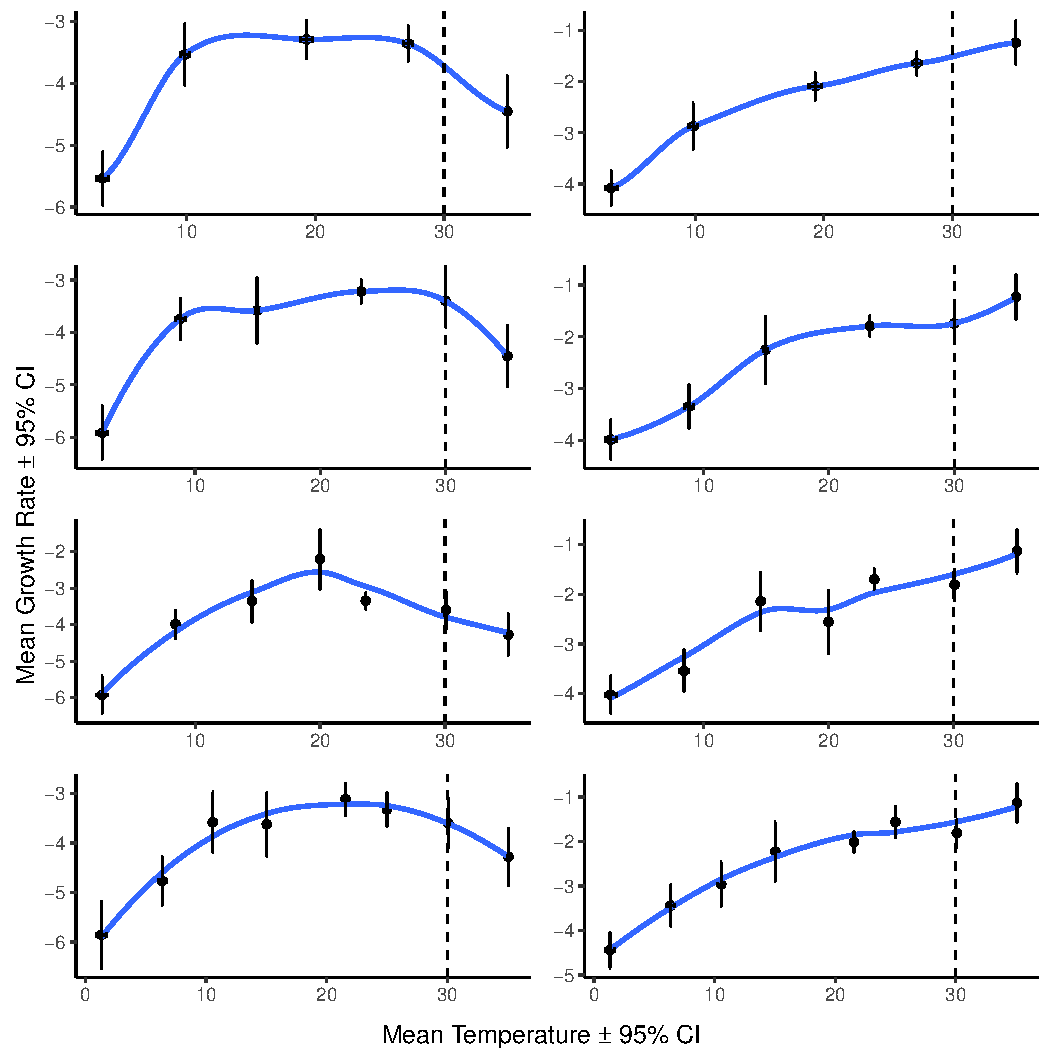
\includegraphics[width=1\textwidth]{Plot/mean_rate_temp_group.pdf}
\caption{Operational Temperature Range Grouped by Temperature}\label{fig:mean_rate_temp_group}
{\footnotesize Across species mean maximum growth rate ($log(r_{max})$, left) and lag phase growth rate ($log(1/t_{lag})$, right) with 95\% confidence interval in different groups of temperature, from the first to the forth row represents 5-8 groups respectively.}
\end{figure}



%%%%%%%%%%%
\subsection{Typical Model Fitting Plot}
\begin{figure}[ht!]
\centering
    \begin{subfigure}{.47\textwidth}
      \centering
      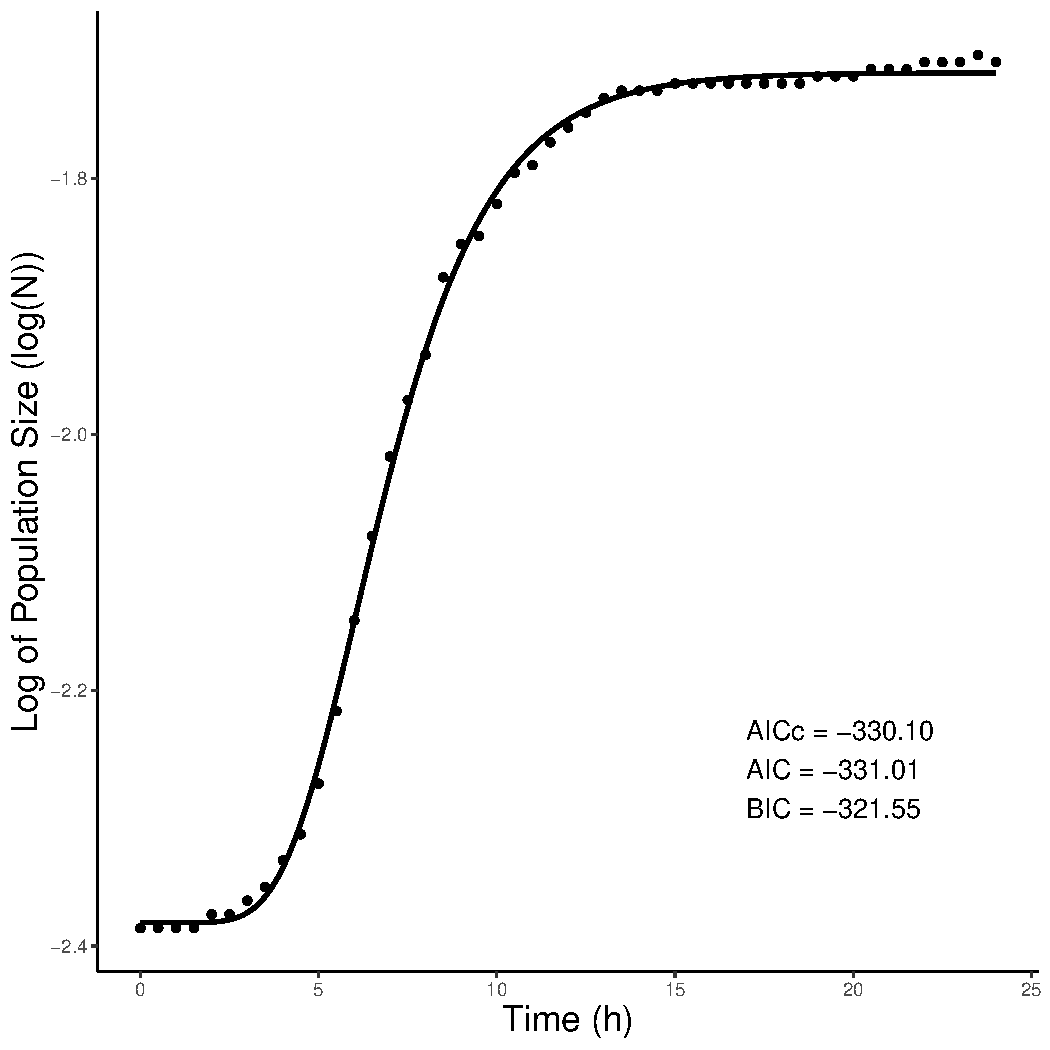
\includegraphics[width=.9\linewidth]{Plot/typ_gomp_fit.pdf}
      \caption{Typical Gompertz Model Fitting Plot}
      \label{fig:typ_gomp_fit}
    \end{subfigure}%
    \begin{subfigure}{.47\textwidth}
      \centering
      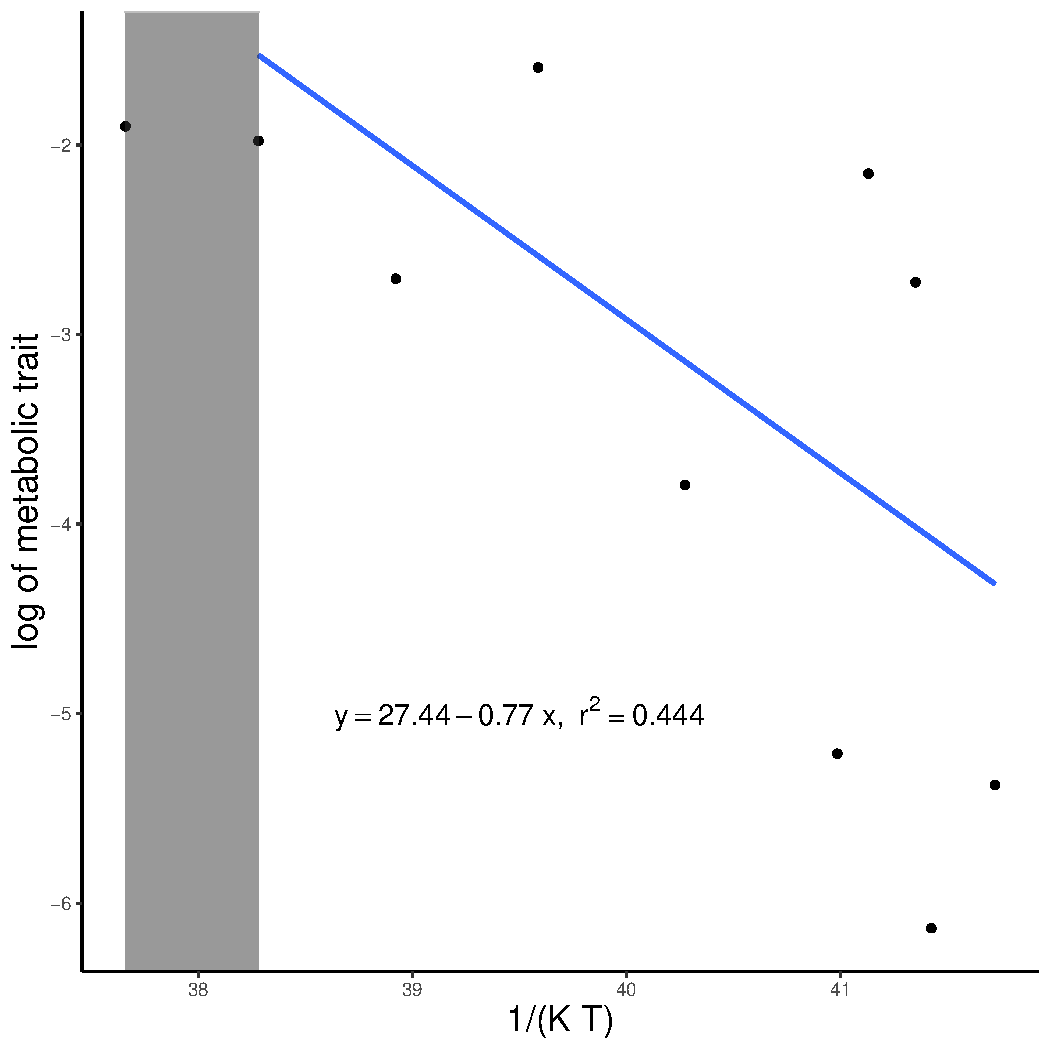
\includegraphics[width=.9\linewidth]{Plot/typ_arrhe_fit.pdf}
      \caption{Typical Boltzmann-Arrhenius Model Fitting Plot}
      \label{fig:typ_arrhe_fit}
    \end{subfigure}

\caption{Typical Model Fitting Plot}\label{fig:typ_fit}
{\footnotesize The typical model fitting plots. \textbf{a} A typical Gompertz Model fitting plot with \textit{AICc, AIC, BIC} as goodness of fit criteria. \textbf{b} A typical Boltzmann-Arrhenius model fitting plot with \textit{$r^2$}}
\end{figure}

%%% Activation Energy
%\newpage
\subsection{Activation Energy}

% figure
%1
\begin{figure}[ht!]
\centering
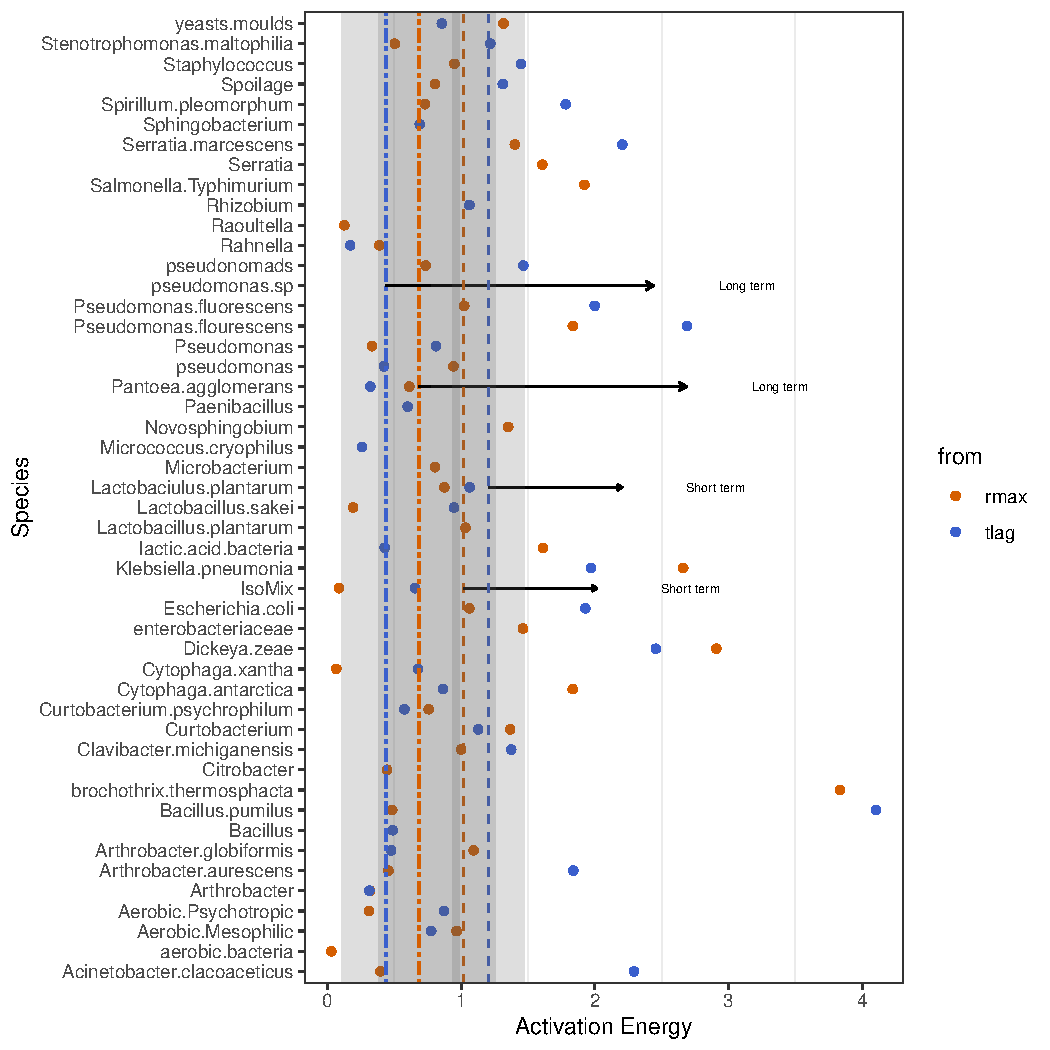
\includegraphics[width=1\linewidth]{Plot/E_spe.pdf}
\caption{Activation Energy of Each Species}\label{fig:E_Spe}
{\footnotesize Variation in short-term thermal sensitivity($E_S$) amongst bacteria groups, with vertical dash lines annotating the mean variations($\Bar{E}_S$, short-term) and the long-term($E_L$) sensitivity both with 95\% confidence interval}
\end{figure}

\begin{center}
% latex table generated in R 4.1.0 by xtable 1.8-4 package
% Sun Aug 15 16:55:43 2021
\begin{table}[ht]
\centering
\begin{tabular}{rlrrr}
  \hline
 & Species & E.value & Confidence.Interval & P.value \\ 
  \hline
1 & Pantoea.agglomerans & 1.1555603903E+00 & 6.2858792339E-01 & 7.8941604021E-03 \\ 
  2 & Clavibacter.michiganensis & 1.2012386963E+00 & 7.2035536371E-01 & 2.0662485300E-02 \\ 
  3 & Stenotrophomonas.maltophilia & 5.4567831439E-01 & 4.4863565962E-01 & 4.1034677993E-02 \\ 
  4 & Bacillus.pumilus & 8.5985176303E-01 & 4.9767234461E-01 & 2.5924118012E-02 \\ 
  5 & Aerobic.Psychotropic & 8.6533345980E-01 & 4.2059531790E-01 & 8.1098910112E-04 \\ 
  6 & Aerobic.Mesophilic & 1.2406834647E+00 & 5.3111010753E-01 & 2.5506125596E-04 \\ 
  7 & Pseudomonas.flourescens & 4.7617684816E+00 & 2.3400073431E+00 & 4.7499765766E-03 \\ 
  8 & pseudomonas & 2.1701790335E+00 & 9.1882632739E-01 & 1.7972884006E-02 \\ 
  9 & Serratia.marcescens & 1.7970209613E+00 & 1.1803257185E+00 & 1.8715688310E-02 \\ 
  10 & Weissella.viridescens & 1.2285562277E+00 & 4.8211259590E-01 & 6.9993952483E-03 \\ 
  11 & Mean Value & 1.5825870793E+00 & 7.5005254309E-01 & 1.4501943621E-02 \\ 
   \hline
\end{tabular}
\end{table}

\end{center}
\begin{center}
% latex table generated in R 4.1.1 by xtable 1.8-4 package
% Sun Aug 22 20:00:15 2021
\begin{table}[ht]
\centering
\begin{tabular}{rlrr}
  \hline
 & Species & E.value & Confidence.Interval \\ 
  \hline
1 & Pantoea.agglomerans & 3.2065484995E-01 & 2.0261744474E+00 \\ 
  2 & Clavibacter.michiganensis & 1.3741532959E+00 & 2.7386069317E+00 \\ 
  3 & Stenotrophomonas.maltophilia & 1.2185292311E+00 & 5.7080248684E-01 \\ 
  4 & Klebsiella.pneumonia & 1.9716850572E+00 & 2.3071507342E+00 \\ 
  5 & Dickeya.zeae & 2.4560490952E+00 & 1.3909428718E+00 \\ 
  6 & Acinetobacter.clacoaceticus & 2.2927193394E+00 & 1.6426021111E+00 \\ 
  7 & Bacillus.pumilus & 4.1038884743E+00 & 2.7852972220E+00 \\ 
  8 & Pseudomonas.fluorescens & 1.9986844721E+00 & 4.5923828736E+00 \\ 
  9 & Staphylococcus & 1.4477321739E+00 & 4.6199587467E-01 \\ 
  10 & Pseudomonas & 8.1156355755E-01 & 2.7860276756E-01 \\ 
  11 & Aerobic.Psychotropic & 8.7054572161E-01 & 4.6369045704E-01 \\ 
  12 & Aerobic.Mesophilic & 7.7598733247E-01 & 5.7124030388E-01 \\ 
  13 & Spoilage & 1.3103794439E+00 & 1.5980454729E+00 \\ 
  14 & Escherichia.coli & 1.9290472286E+00 & 3.9536563108E+00 \\ 
  15 & Curtobacterium.psychrophilum & 5.7547281206E-01 & 8.2534829665E-01 \\ 
  16 & Cytophaga.antarctica & 8.6434179183E-01 & 5.6319675635E-01 \\ 
  17 & Cytophaga.xantha & 6.7703430495E-01 & 8.1564499817E-01 \\ 
  18 & Spirillum.pleomorphum & 1.7815692937E+00 & 8.7011892340E-01 \\ 
  19 & Micrococcus.cryophilus & 2.5849023891E-01 & 1.0705993267E+00 \\ 
  20 & Pseudomonas.flourescens & 2.6879164913E+00 & 2.7824753536E+00 \\ 
  21 & pseudomonas & 4.2227309562E-01 & 1.2827742161E+00 \\ 
  22 & yeasts.moulds & 8.5506851885E-01 & 1.6072729184E+00 \\ 
  23 & lactic.acid.bacteria & 4.2770108072E-01 & 2.5827988171E+00 \\ 
  24 & pseudonomads & 1.4648694644E+00 & 1.4386373967E+00 \\ 
  25 & Serratia.marcescens & 2.2052486393E+00 & 1.2403294563E+00 \\ 
  26 & Arthrobacter & 3.1328343052E-01 & 5.8346638330E-01 \\ 
  27 & Arthrobacter.aurescens & 1.8386360620E+00 & 1.7373564498E-01 \\ 
  28 & Arthrobacter.globiformis & 4.7629968860E-01 & 1.4098413475E+00 \\ 
  29 & Lactobacillus.sakei & 9.4621117146E-01 & 1.0086183868E+00 \\ 
  30 & Lactobaciulus.plantarum & 1.0642098106E+00 & 6.2787266075E-01 \\ 
  31 & Rahnella & 1.6967053479E-01 & 7.9940640337E-01 \\ 
  32 & Sphingobacterium & 6.9031618237E-01 & 1.7921975981E+00 \\ 
  33 & Rhizobium & 1.0610503552E+00 & 9.5983883501E-01 \\ 
  34 & Curtobacterium & 1.1268698833E+00 & 1.3894959862E+00 \\ 
  35 & IsoMix & 6.5587897228E-01 & 6.0147066300E-01 \\ 
  36 & Paenibacillus & 5.9979189848E-01 & 1.1831431247E+00 \\ 
  37 & Bacillus & 4.8855399057E-01 & 1.5725434047E+00 \\ 
  38 & Mean Value & 1.2035777564E+00 & 2.6964036944E-01 \\ 
   \hline
\end{tabular}
\end{table}

\end{center}

